\documentclass[12pt,a4paper]{article}
\usepackage{physics}
\usepackage{amssymb}
\usepackage{subcaption}
\usepackage{colortbl}
\newcommand{\activity}{Activity 6 -- Color Order System}
\input{spp.dat}

%  Editorial staff will uncomment the next line
% \providecommand{\artnum}[0]{XX-XX}
% \renewcommand{\articlenum}[0]{SPP-\the\year-\artnum-}

\begin{document}

\title{\TitleFont \activity}
\author[ ]{\textbf{Kenneth V. Domingo} \\
2015--03116 \\
App Physics 187, 1\textsuperscript{st} Semester, A.Y. 2019--20}
\affil[ ]{\corremail{kvdomingo@up.edu.ph} }

\maketitle
\thispagestyle{titlestyle}

\section*{Results and Discussion}
\setcounter{section}{1}

For this activity, the CIE 1964 standard observer values for 380--780 nm was obtained from \cite{cie64}. The tristimulus values were calculated using \cite{soriano}

\begin{align}
	X &= \int P(\lambda) \bar{x}(\lambda) \dd{\lambda} \nonumber \\
	Y &= \int P(\lambda) \bar{y}(\lambda) \dd{\lambda} \label{eq:tristimulus} \\
	Z &= \int P(\lambda) \bar{z}(\lambda) \dd{\lambda} \nonumber
\end{align}

\noindent
Their $xy$ coordinates were obtained by normalizing each value by their sum. Figure \ref{fig:locus} shows the obtained boundaries for the CIE tongue by considering monochromatic lights ($P(\lambda) = \delta(\lambda)$). The Planckian locus was obtained by substituting into $P(\lambda)$ the spectral radiant exitance for a blackbody, given by

\begin{equation}\label{eq:planck}
	M(\lambda, T) = \frac{2\pi hc^2}{\lambda^5} \frac{1}{\exp[\frac{hc}{k\lambda T}] - 1}
\end{equation}

\begin{figure}[htb]
	\centering
	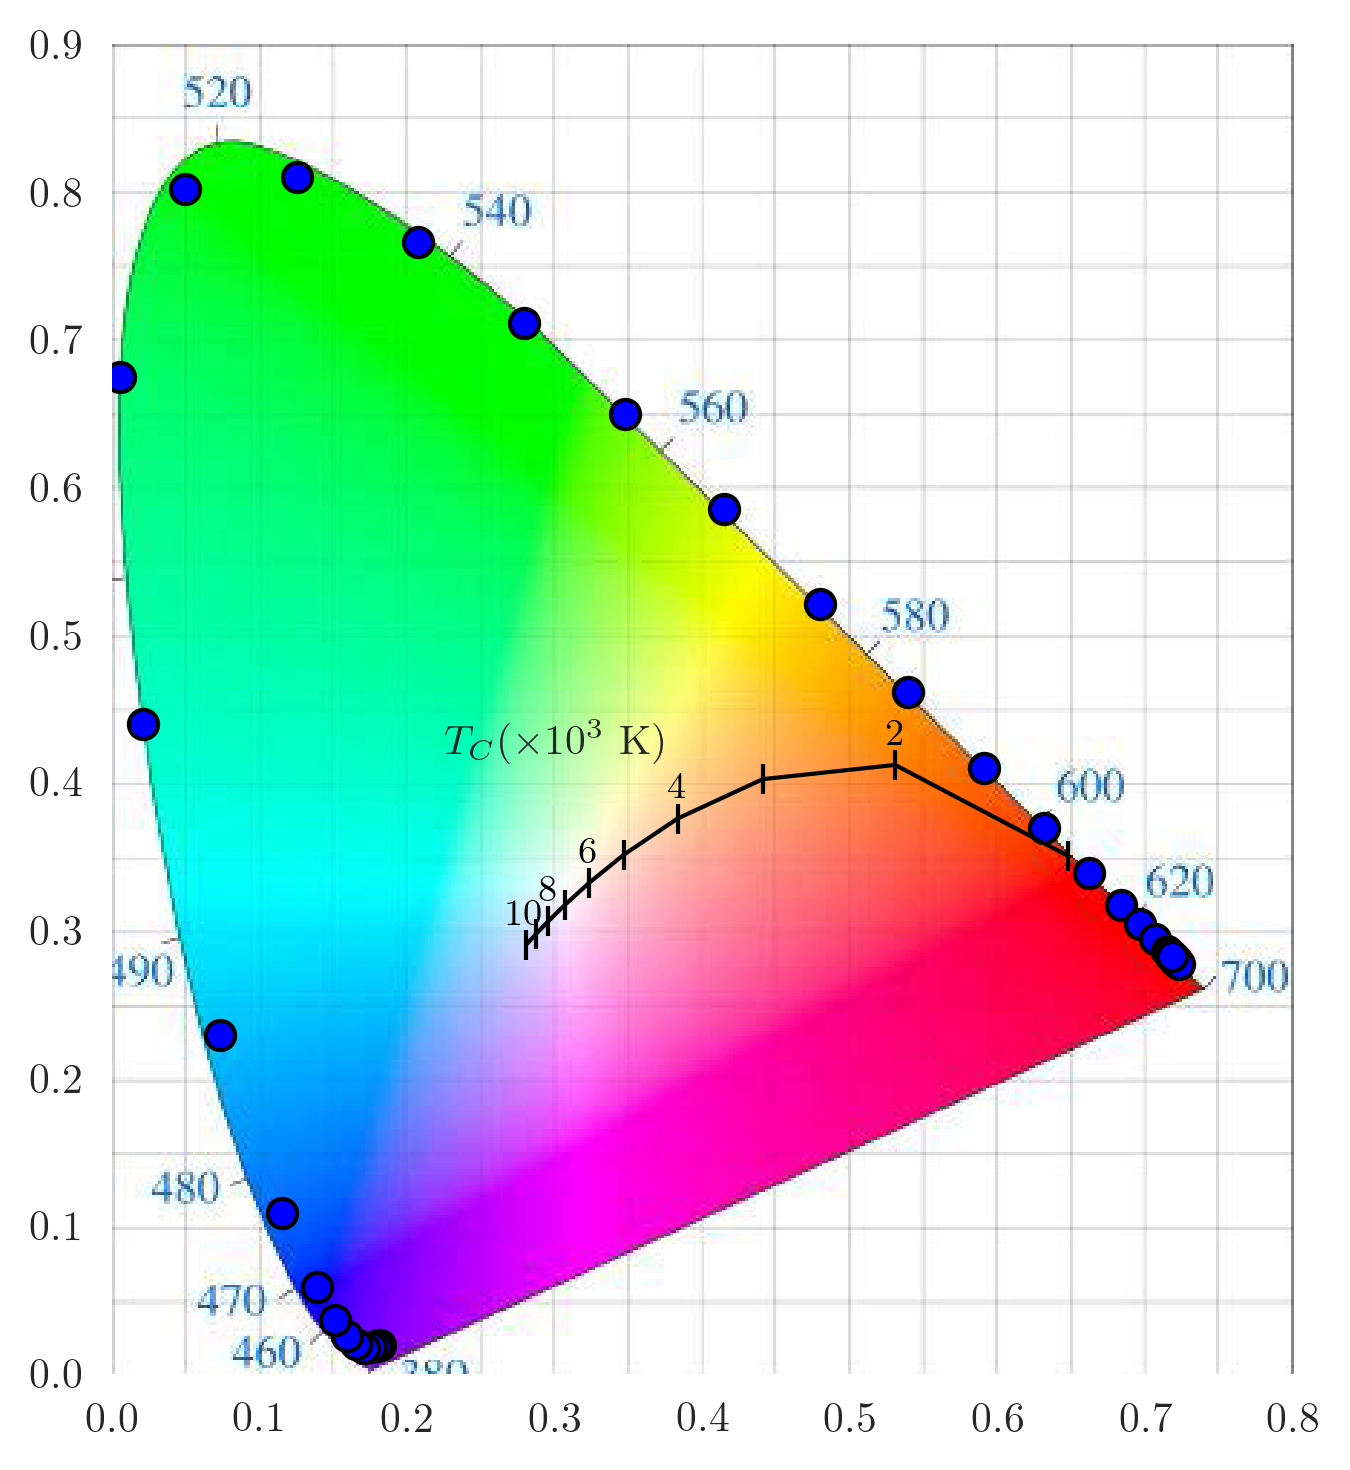
\includegraphics[width=0.65\textwidth]{locus.png}
	\caption{Calculated boundaries of the CIE tongue (blue circles), and the associated Planckian locus (black spines).}
	\label{fig:locus}
\end{figure}

\bibliographystyle{spp-bst}
\bibliography{biblio}

\end{document}